%%%%%%%%%%%%
%
% $Autor: Chantal Crety $
% $Datum: 11.07.2025 $
% $Pfad: DemonstratorSchrittmotor\MontageAnleitung\Bauteile.tex
% $Beschreibung: Materialliste der MontageAnleitung
%
%%%%%%%%%%%%

\chapter{Materialliste}

\textbf{Material:}
In der Tabelle 2.1 werden alle Bauteile gezeigt und anschließend für einen einfacheren Aufbau in die Tabellen Elektrische Komponenten \ref{EKomponenten} und Verbindungskomponenten \ref{VKomponenten} aufgeteilt. \\

\textbf{Werkzeug:}
Bei den benötigten Werkzeugen für die Montage handelt es sich um einen Seitenschneider, Lötkolben, sowie einen 3D-Drucker. Beide Geräte können nach Recherche in Community Werkstätten genutzt werden. 

\begin{center}
	\scriptsize
	\begin{longtable}{|c|c|p{2.5cm}|p{2cm}|p{0.8cm}|c|p{2cm}|}
		
		\hline
		\textbf{Pos.} & \textbf{Stk.} & \textbf{Bezeichnung} & \textbf{Artikel-Nr.} & \textbf{Preis [€]} & \textbf{Abbildung} & \textbf{Bestelladresse} \\
		\hline
		1 & 1 & Genmitsu 3018 Pro CNC Fräsemachine & 101-60-280PRO & 219,00  & 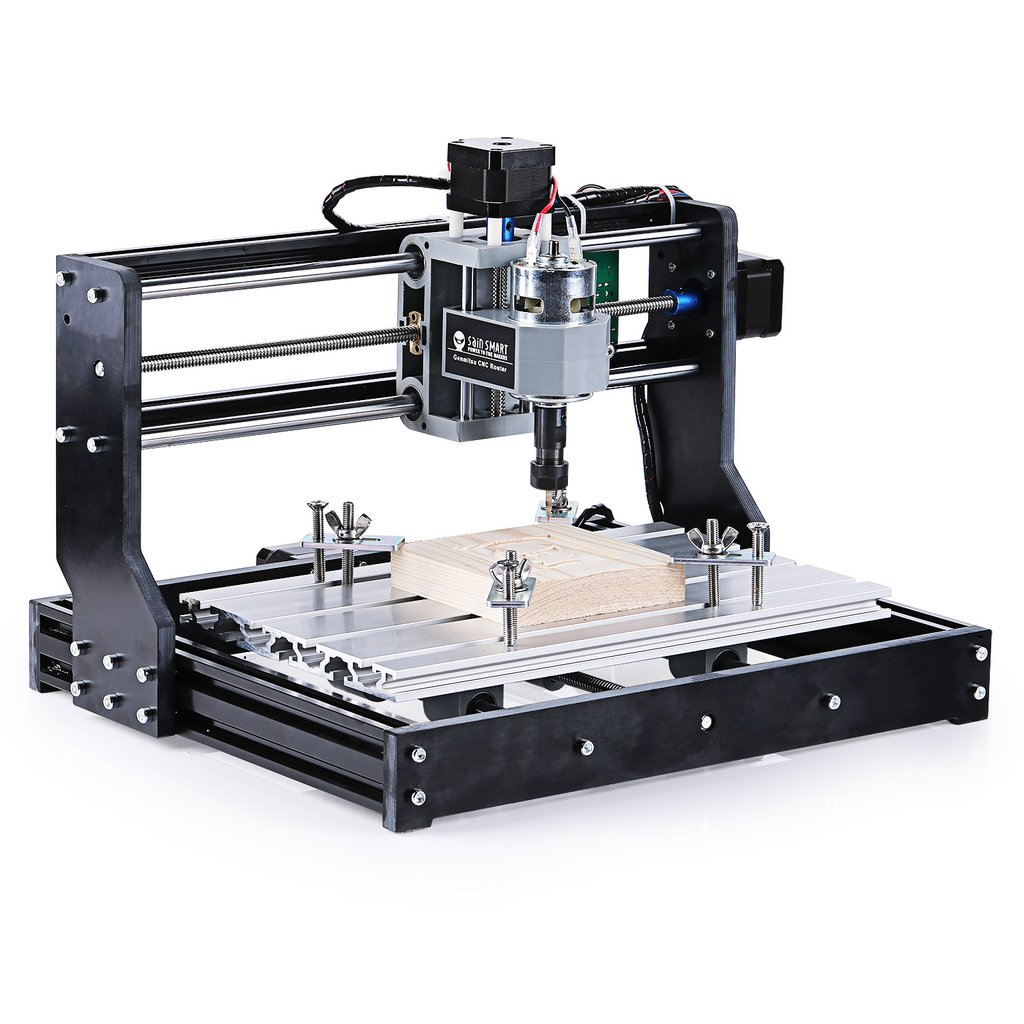
\includegraphics[width=1.5cm]{Images/fraesmaschine.jpg}
		& \url{www.amazon.de} \\
		\hline
		2 & 1 & Arduino Nano 33 BLE Sense Rev.2\newline nRF52840, mit Header& ARD NANO 33BSH2 & 47,70 & 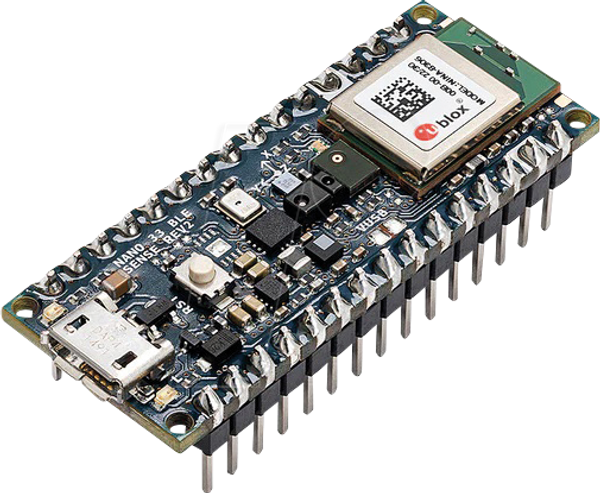
\includegraphics[width=1.5cm]{Images/arduino.png} & \url{www.reichelt.de} \\
		\hline
		5 & 1 & 65 Jumper Wire Kabel im Set & RBS10022 & 1,55 & 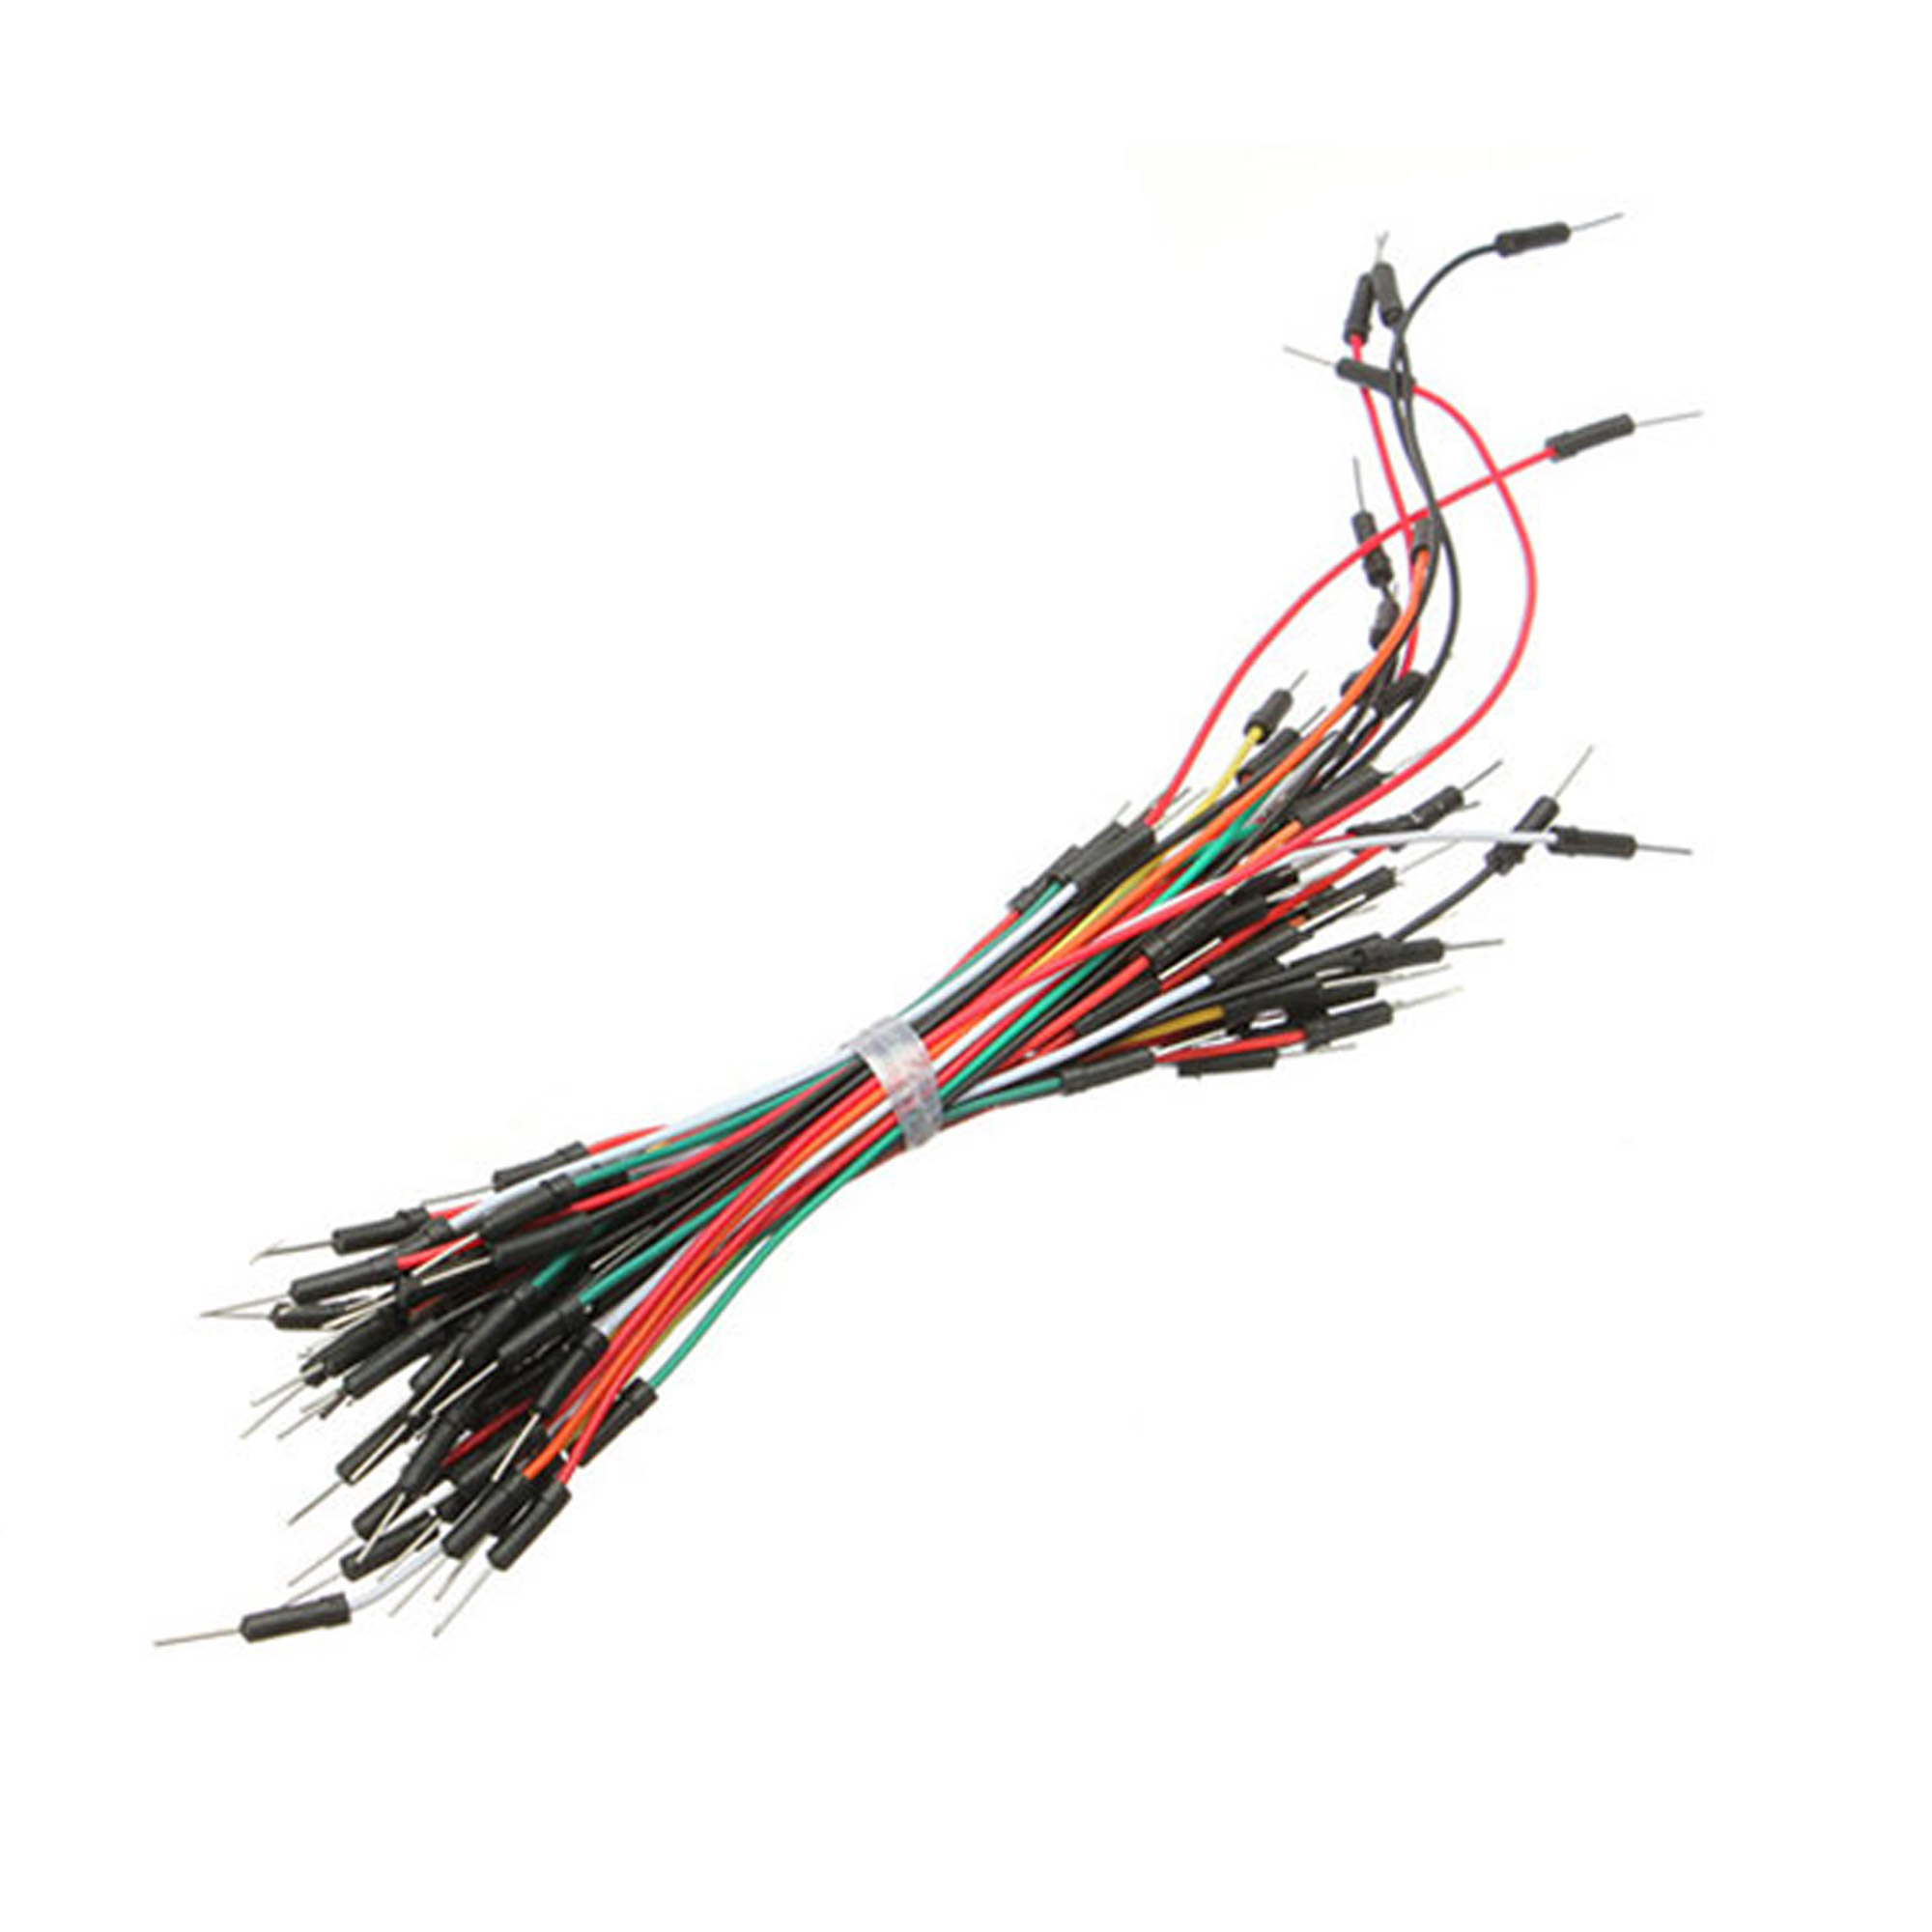
\includegraphics[width=1.5cm]{Images/jumpercablemm.jpg} & \url{www.roboter-bausatz.de} \\
		\hline
		4 & 1 & 40 Pin Dupont / Jumper Kabel Buchse-Buchse 20 cm & RBS101126 & 0,98 & 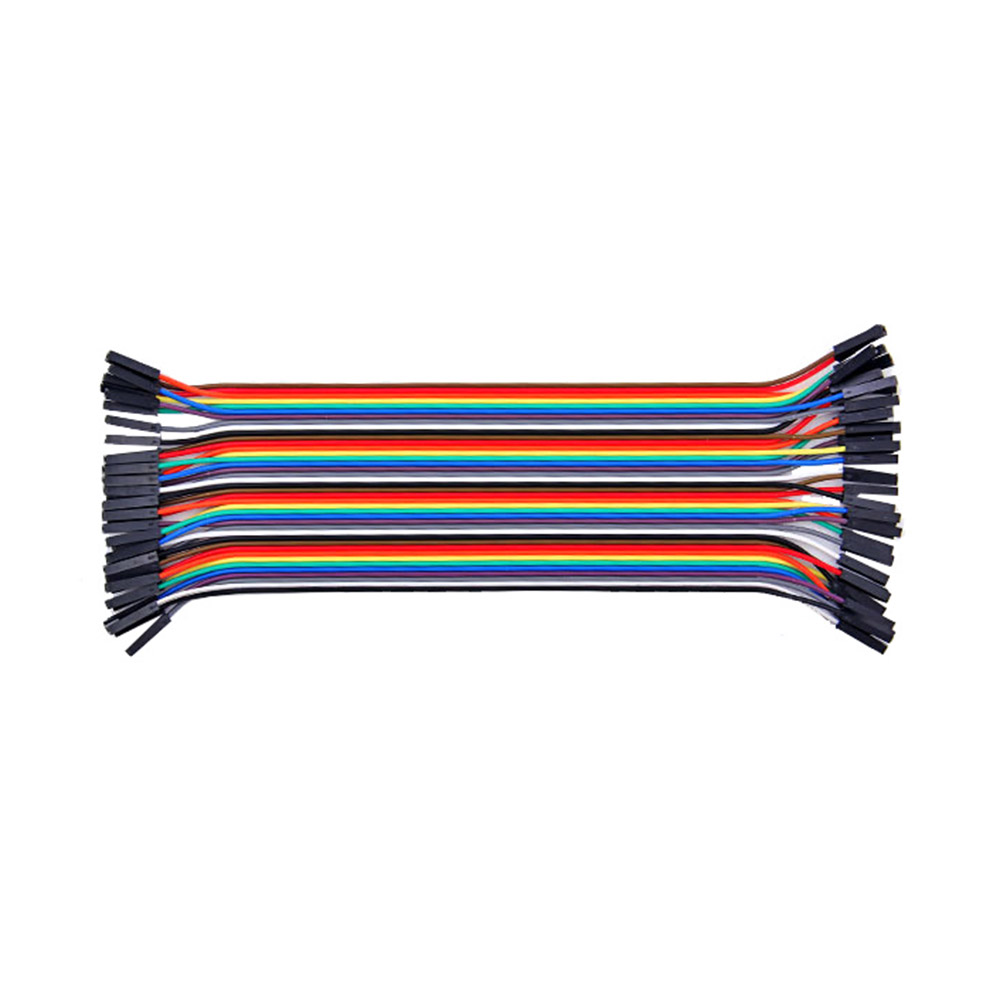
\includegraphics[width=1.5cm]{Images/jumpercableff.jpg} & \url{www.roboter-bausatz.de} \\
		\hline
		5 & 1 & 40 Pin Jumper Kabel Buchse-Stecker 20 cm & RBS10028 & 1,15 & 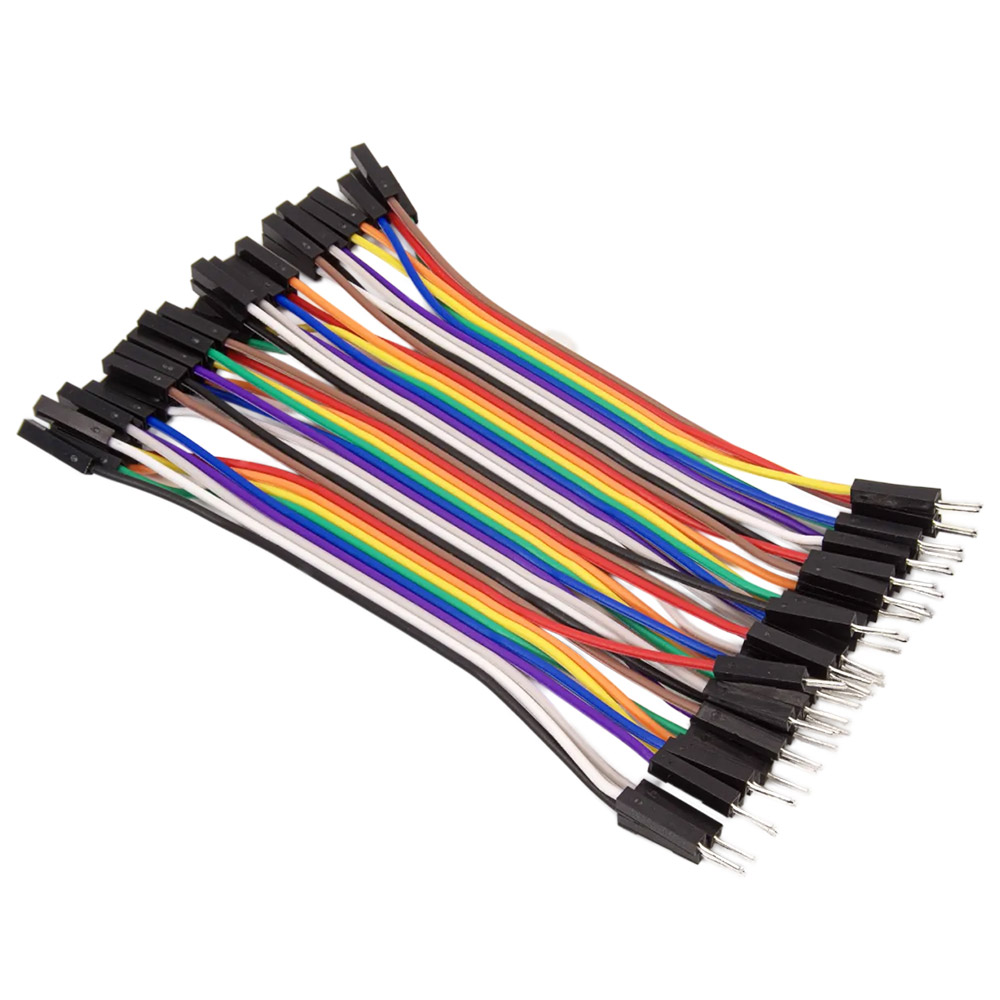
\includegraphics[width=1.5cm]{Images/jumpercablemf.jpg} & \url{www.roboter-bausatz.de} \\
		\hline
		6 & 1 & Arduino - Grove Universal-Kabel, 4-Pin, 20 cm & GRV CA-BLE4PIN20 & 2,50 & 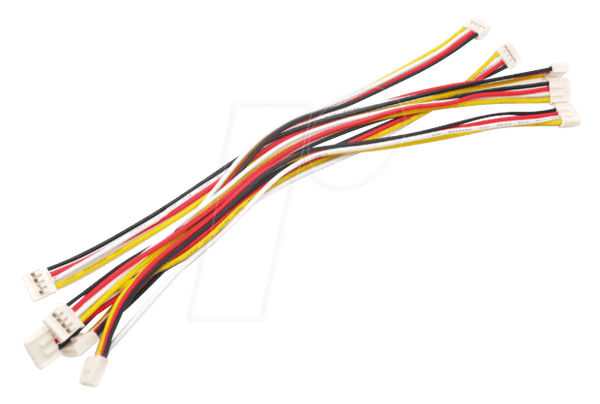
\includegraphics[width=1.5cm]{Images/grove2.png} & \url{www.reichelt.de} \\
		\hline
		7 & 1 & TRU COMPONENTS DC-13M Niedervolt-Steckverbinder Stecker, gerade 5.5 mm 2.5 mm 1 St. & 1572162 - VQ & 3,79 & 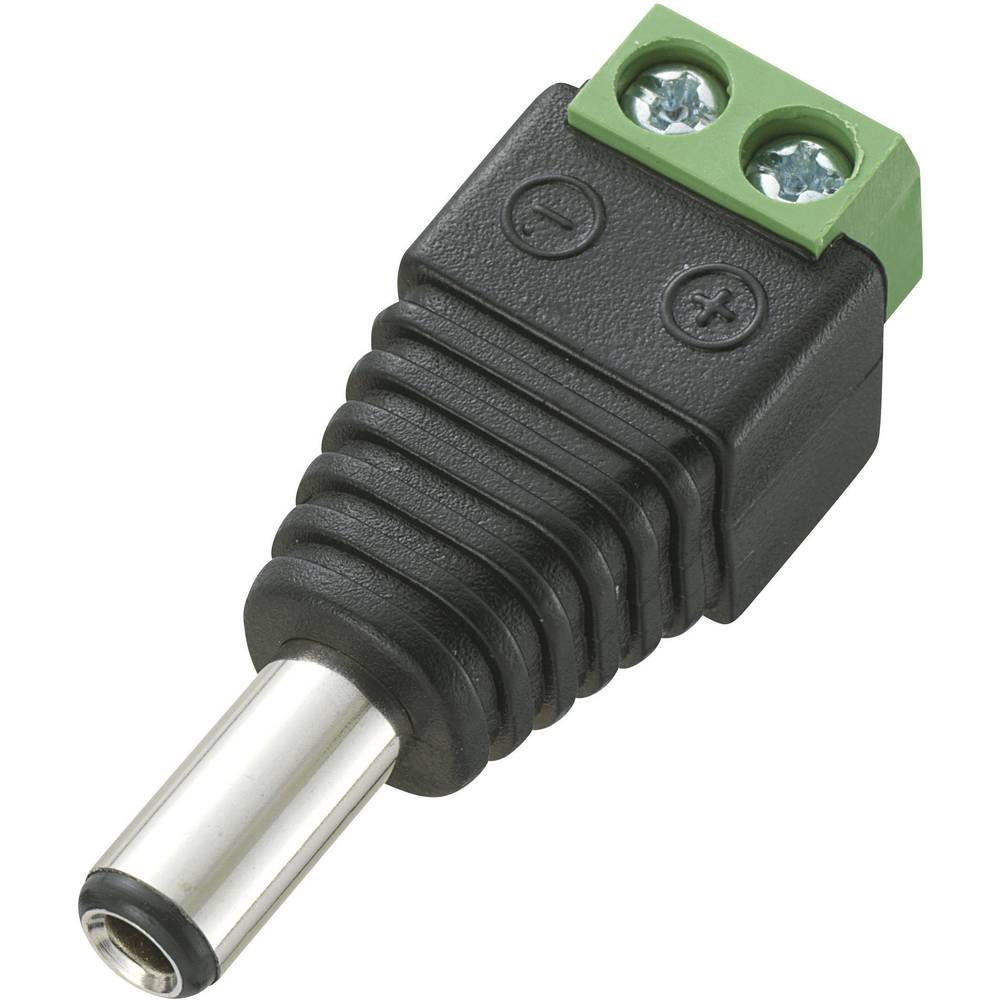
\includegraphics[width=1.5cm]{Images/schutzstecker.jpg} & \url{www.conrad.de} \\
		\hline
		8 & 1 & Steckernetzteil, 12 W, 12 V, 1 A & NKSK 200 SW GEW & 3,10 & 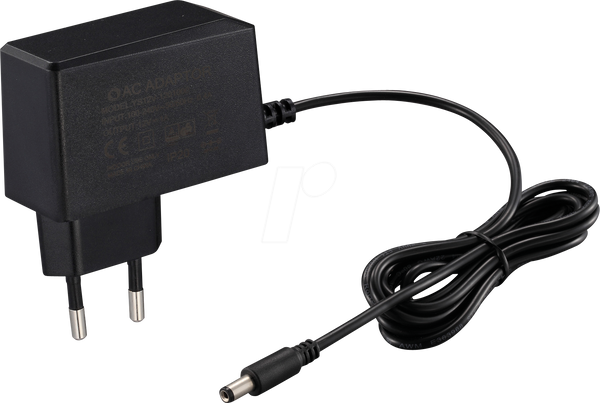
\includegraphics[width=1.5cm]{Images/netzteil.png} & \url{www.reichelt.de} \\
		\hline
		9 & 1 & Drucktaster 0,1A-24VAC 1x (Ein) Ø11/9,1mm rt & RAFI 107.301 & 2,99 & 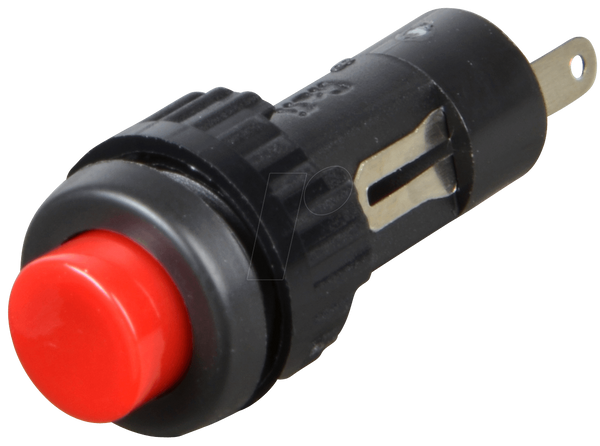
\includegraphics[width=1.5cm]{Images/tasterr.png} & \url{www.reichelt.de} \\
		\hline
		10 & 1 & Drucktaster 0,1A-24VAC 1x (Ein) Ø11/9,1mm gn & RAFI 107.507
		& 2,90 & 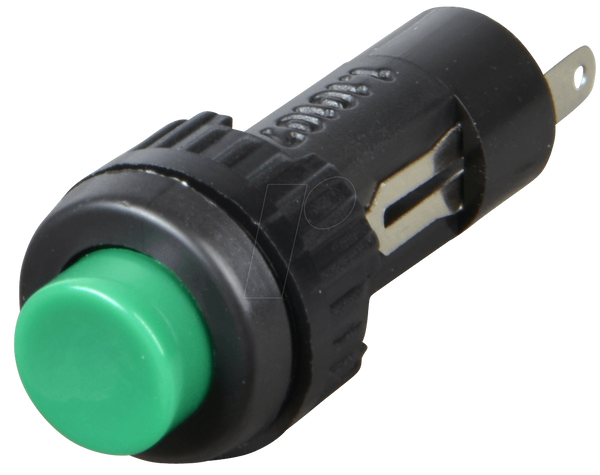
\includegraphics[width=1.5cm]{Images/tasterg.png} & \url{www.reichelt.de} \\
		\hline
		11 & 2 & Snap-Action-Mikroschalter, 1x UM, Rollenhebel & AV 32543 AT & 1,80 & 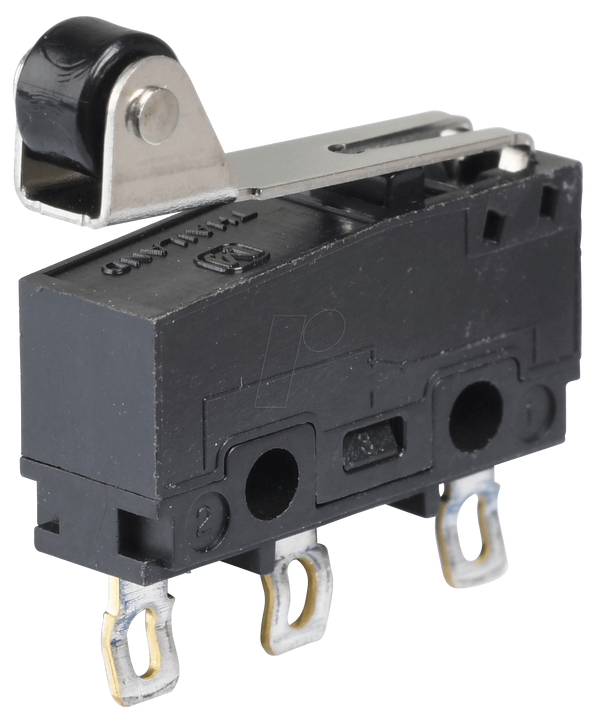
\includegraphics[width=1.5cm]{Images/microschalter.png} & \url{www.reichelt.de} \\
		\hline
		12 & 1 & Entwicklungsboard mit DRV8825 Motortreiber & DEBO DRV A4988 & 5,80 & 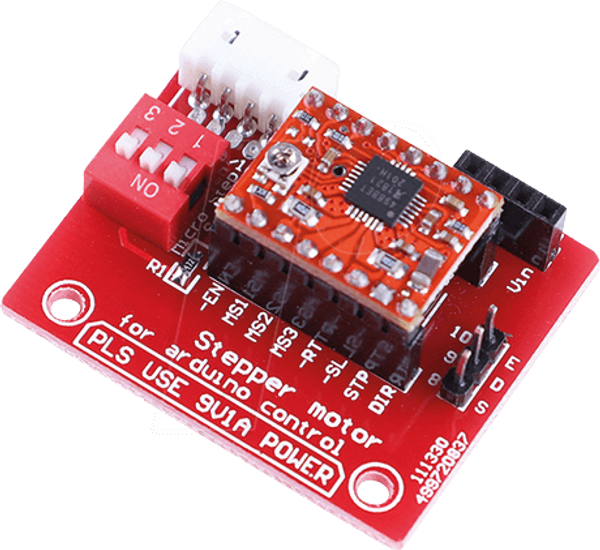
\includegraphics[width=1.5cm]{Images/treiber.png} & \url{www.reichelt.de} \\
		\hline
		13 & 1 & Entwicklerboards - Display OLED, 2,42", 128x64 Pixel & DEBO OLED 2.42 & 18,90 & 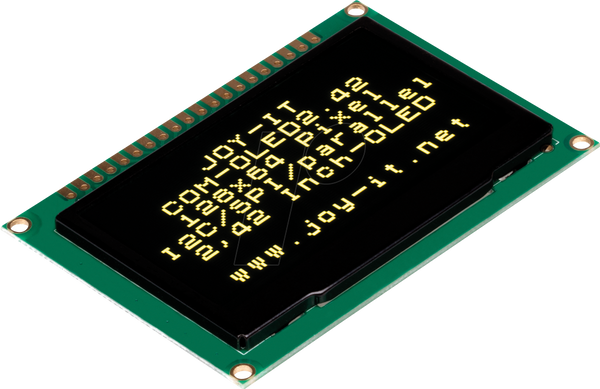
\includegraphics[width=1.5cm]{Images/display.png} & \url{www.reichelt.de} \\
		\hline
		14 & 1 & Sunlu PLA Filament 0.75mm 1kg & RBS16624 & 17,95 & 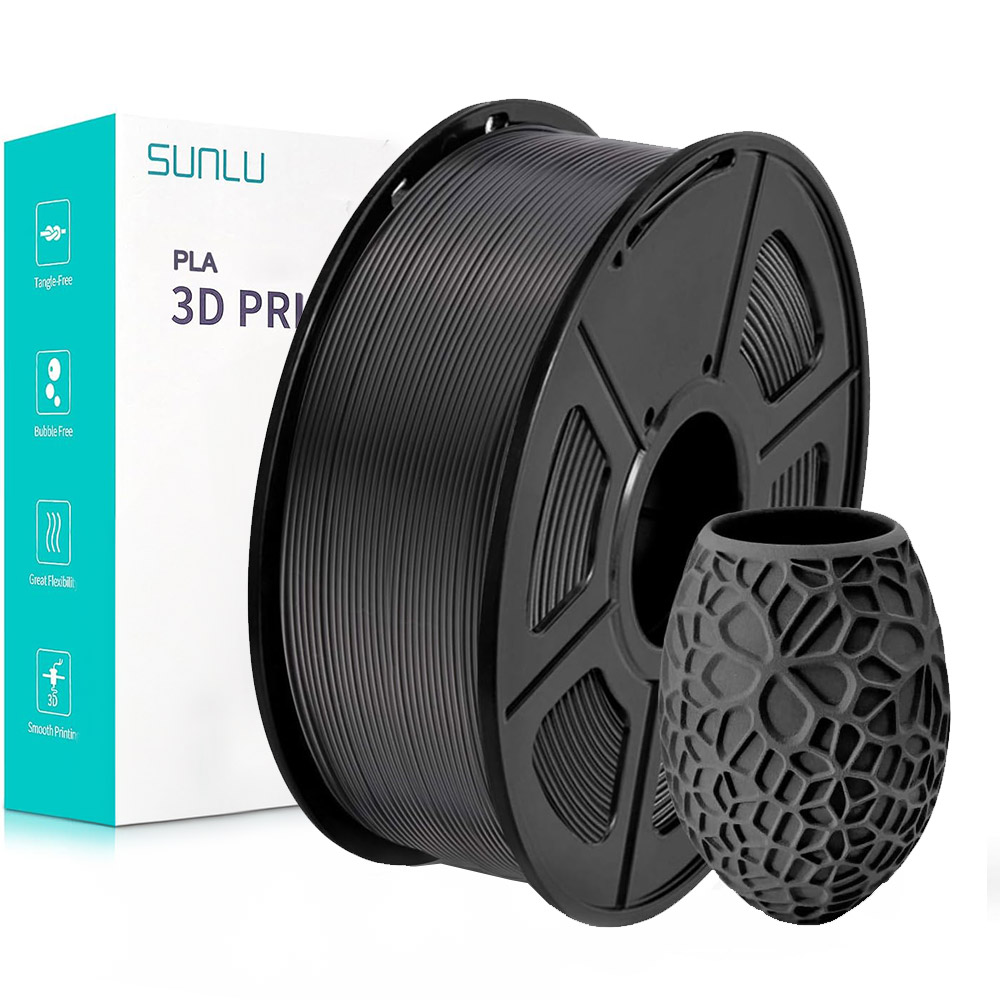
\includegraphics[width=1.5cm]{Images/filament.jpg} & \url{www.roboter-bausatz.de} \\
		\hline
		15 & 1 & Experimentier-Slide-Steckboard, 300/100 Kontakte & STECKBOARD S4 & 4,20 & 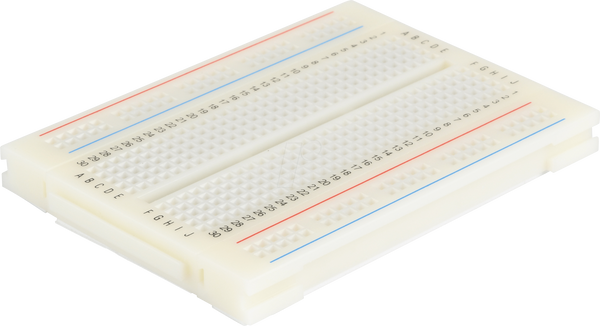
\includegraphics[width=1.5cm]{Images/breadboard.png} & \url{www.reichelt.de} \\
		\hline
		16 & 1 & Kabelbinder-Set, verschiedene Größen, mehrfarbig, 200er-Pack & DELOCK 18628 & 3,85 & 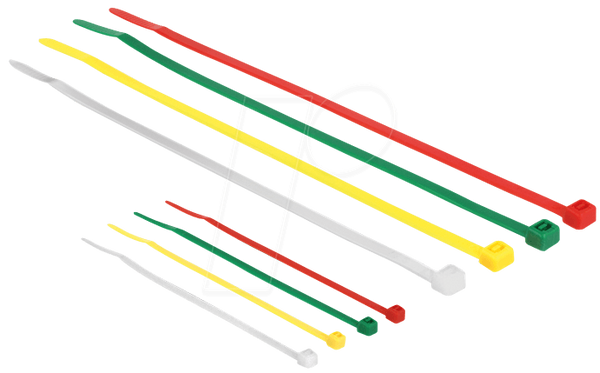
\includegraphics[width=1.5cm]{Images/kabelbinder.png} & \url{www.reichelt.de} \\
		\hline
		17 & 1 & Drehwinkel-Encoder, KY-040 & DEBO ENCODER & 2,20 & 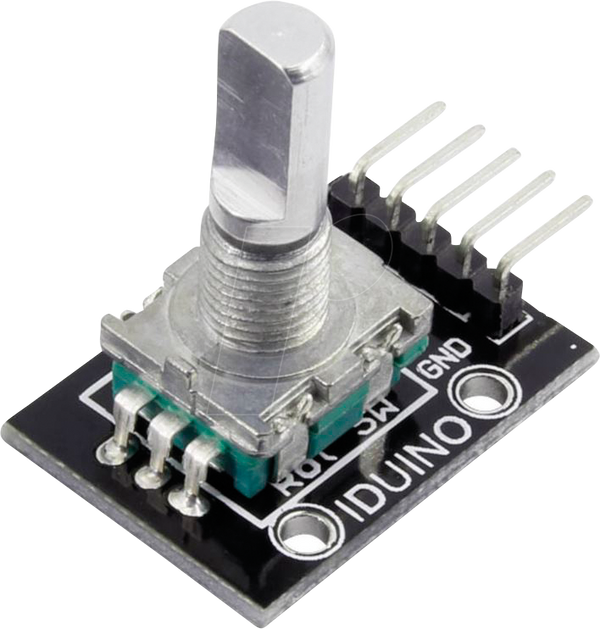
\includegraphics[width=1.5cm]{Images/drehknopf.png} & \url{www.reichelt.de} \\
		\hline
		18 & 1 & Wippschalter, 2x Aus, schwarz, I-O & WIPPE 1858.1103 & 2,60 & 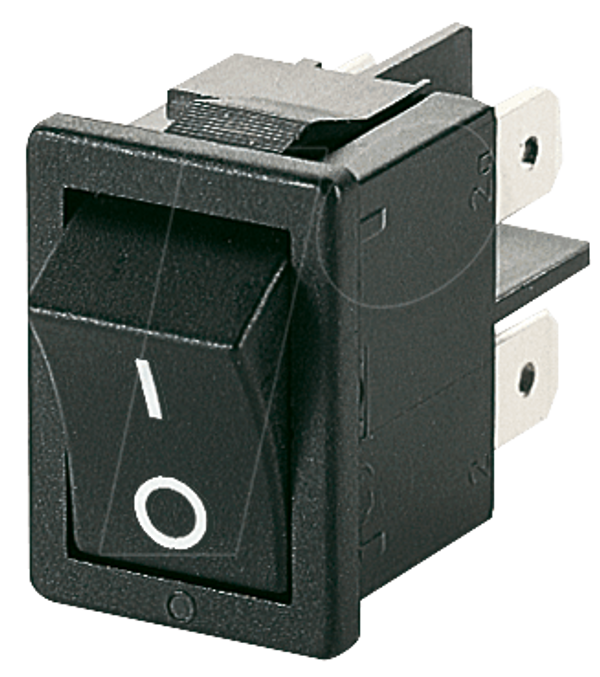
\includegraphics[width=1.5cm]{Images/wippschalter.png} & \url{www.reichelt.de} \\
		\hline
		19 & 1 & Zylinderkopfschraube, Sechskantschraube, M5, 10 mm & ZS M5X10 & 0,30 & 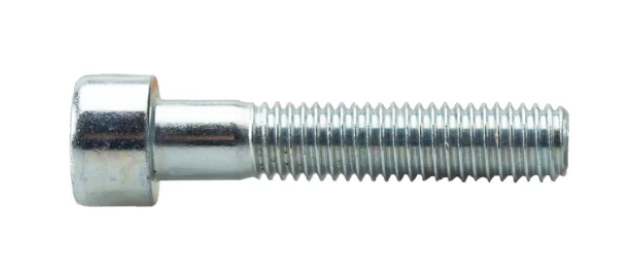
\includegraphics[width=1.5cm]{Images/zylinderkopfschraube.png} & \url{www.reichelt.de} \\
		\hline
		20 & 3 & Flach-Senkkopfschrauben, Kreuzschlitz, M3, 10 mm & SKS M3X10-50 & 1,75 & 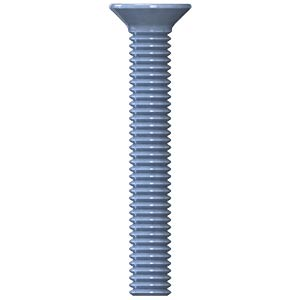
\includegraphics[width=1.5cm]{Images/senkkopfschraube.jpg} & \url{www.reichelt.de} \\
		\hline
		21 & 3 & Sechskantmuttern, Edelstahl A2, M3 & SK-E M3-100 & 4,55 & 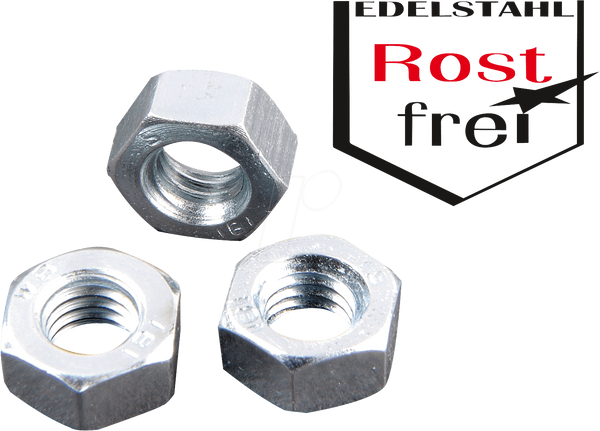
\includegraphics[width=1.5cm]{Images/muttern.png} & \url{www.reichelt.de} \\
		\hline	
		22 & 1& Unterlegscheiben, 10,5 mm & SKU 10,5-100 & 5,35 & 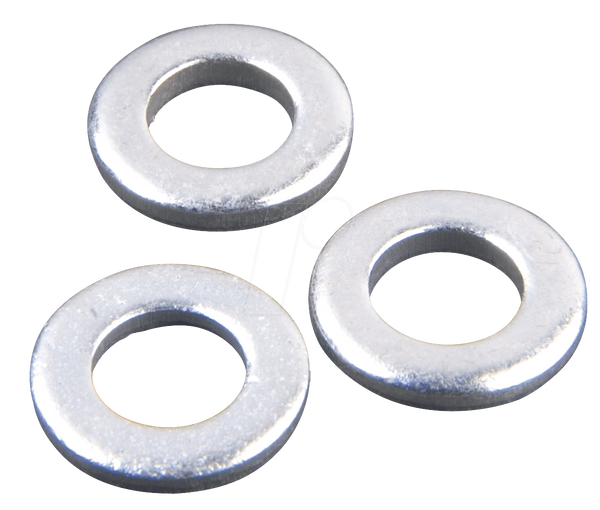
\includegraphics[width=1.5cm]{Images/unterlegscheibe.png} & \url{www.reichelt.de} \\
		\hline
		23 & 1& Elektroniklot EL 324 bleifrei 70 g & CFH 52324 & 10,99 & 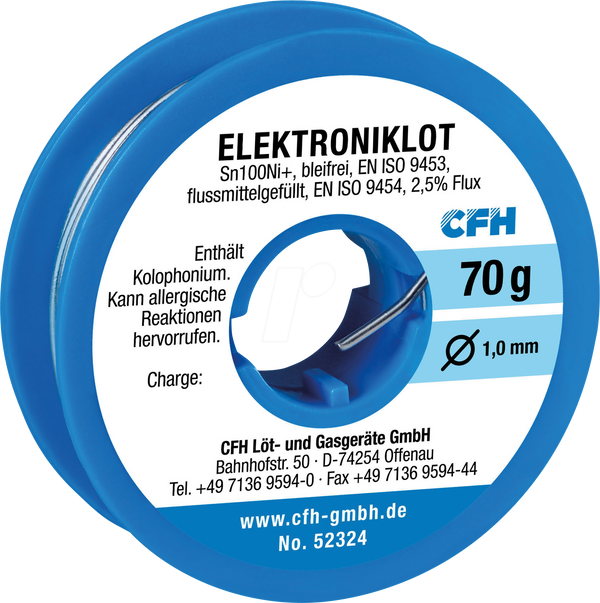
\includegraphics[width=1.5cm]{Images/loetzinn.png} & \url{www.reichelt.de} \\
		\hline	
		
		\caption{Gesamtliste}
		\label{tab:Gesamtliste}
		
	\end{longtable}
\end{center}

\begin{figure}[H]
	\begin{center}
		\fontsize{8}{10}\selectfont
		\begin{tabularx}{\textwidth}{|p{0.4cm}|X|X|X|X|X|} 
			\hline 
			\textbf{Pos.} &  \textbf{Benennung} \\ \hline
			1 & Genmitsu 3018 Pro  \\ \hline
			2 & Arduino Nano 33 BLE Sense   \\ \hline
			3 & Steckernetzteil   \\ \hline
			4 & Entwicklerboard mit DRV8825 Motortreiber   \\ \hline
			5 & Drehwinkel-Encoder  \\ \hline
			6 & OLED-Display  \\ \hline
			7 & Snap-Action-Mikroschalter  \\ \hline
			8 & Drucktaster rot \\ \hline
			9 & Drucktaster grün  \\ \hline
			10 & Wippschalter  \\ \hline
			
		\end{tabularx}
		\captionof{table}{Elektrische Komponenten}	\label{EKomponenten}
	\end{center}
\end{figure}


\begin{figure}[H]
	\begin{center}
		\fontsize{8}{10}\selectfont
		\begin{tabularx}{\textwidth}{|p{0.4cm}|X|X|X|X|X|}  
			\hline 
			\textbf{Pos.} &  \textbf{Benennung} \\ \hline
			1 & Jumper Kabel  \\ \hline
			2 & Grove Kabel  \\ \hline
			3 & Steckerverbinder \\ \hline
			4 & USB-A, Mini-USB Kabel   \\ \hline
			5 & Steckbrett \\ \hline
			6 & Zylinderkopfschraube \\ \hline
			7 & Senkkopfschrauben \\ \hline
			8 & Muttern \\ \hline
			9 & Unterlegscheiben \\ \hline
			10 & Lötzinn \\ \hline
			
		\end{tabularx}
		\captionof{table}{Verbindungskomponenten}	\label{VKomponenten}
	\end{center}
\end{figure}


